% Created 2021-09-27 Mon 12:01
% Intended LaTeX compiler: xelatex
\documentclass[letterpaper]{article}
\usepackage{graphicx}
\usepackage{grffile}
\usepackage{longtable}
\usepackage{wrapfig}
\usepackage{rotating}
\usepackage[normalem]{ulem}
\usepackage{amsmath}
\usepackage{textcomp}
\usepackage{amssymb}
\usepackage{capt-of}
\usepackage{hyperref}
\setlength{\parindent}{0pt}
\usepackage[margin=1in]{geometry}
\usepackage{fontspec}
\usepackage{svg}
\usepackage{cancel}
\usepackage{indentfirst}
\setmainfont[ItalicFont = LiberationSans-Italic, BoldFont = LiberationSans-Bold, BoldItalicFont = LiberationSans-BoldItalic]{LiberationSans}
\newfontfamily\NHLight[ItalicFont = LiberationSansNarrow-Italic, BoldFont       = LiberationSansNarrow-Bold, BoldItalicFont = LiberationSansNarrow-BoldItalic]{LiberationSansNarrow}
\newcommand\textrmlf[1]{{\NHLight#1}}
\newcommand\textitlf[1]{{\NHLight\itshape#1}}
\let\textbflf\textrm
\newcommand\textulf[1]{{\NHLight\bfseries#1}}
\newcommand\textuitlf[1]{{\NHLight\bfseries\itshape#1}}
\usepackage{fancyhdr}
\pagestyle{fancy}
\usepackage{titlesec}
\usepackage{titling}
\makeatletter
\lhead{\textbf{\@title}}
\makeatother
\rhead{\textrmlf{Compiled} \today}
\lfoot{\theauthor\ \textbullet \ \textbf{2021-2022}}
\cfoot{}
\rfoot{\textrmlf{Page} \thepage}
\renewcommand{\tableofcontents}{}
\titleformat{\section} {\Large} {\textrmlf{\thesection} {|}} {0.3em} {\textbf}
\titleformat{\subsection} {\large} {\textrmlf{\thesubsection} {|}} {0.2em} {\textbf}
\titleformat{\subsubsection} {\large} {\textrmlf{\thesubsubsection} {|}} {0.1em} {\textbf}
\setlength{\parskip}{0.45em}
\renewcommand\maketitle{}
\author{Houjun Liu}
\date{\today}
\title{Entropy}
\hypersetup{
 pdfauthor={Houjun Liu},
 pdftitle={Entropy},
 pdfkeywords={},
 pdfsubject={},
 pdfcreator={Emacs 28.0.50 (Org mode 9.4.4)}, 
 pdflang={English}}
\begin{document}

\tableofcontents



\section{Entropy}
\label{sec:org0d9d4fd}
\#flo \#disorganized

Startistical measure of randomness in a reaction of systems.

Entropy measured in microstates --- the spead of energy in states.
Greater numbers of microstates means that there is more entropy

To think about this, think about states of matter:

\begin{itemize}
\item Gas => Most Entropy
\item Water => Meh Entropy
\item Solids => Least Entropy
\end{itemize}

\begin{figure}[htbp]
\centering
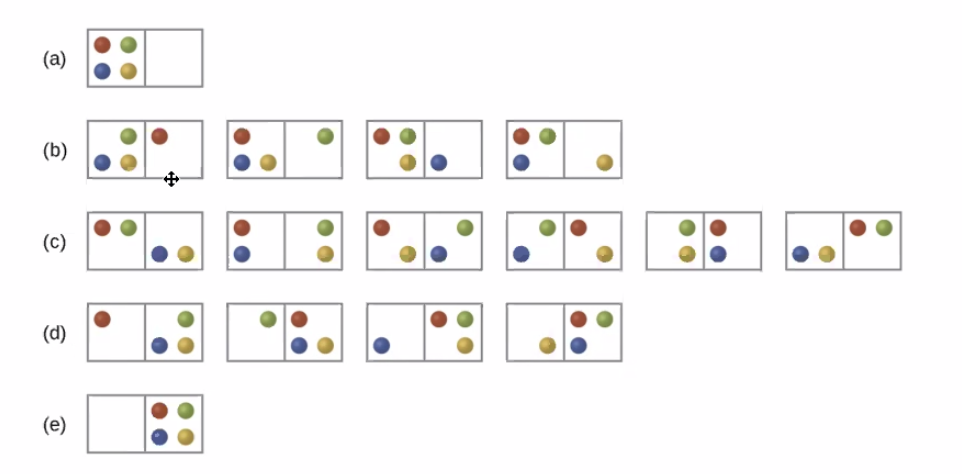
\includegraphics[width=.9\linewidth]{Screen Shot 2020-10-02 at 2.29.24 PM.png}
\caption{Screen Shot 2020-10-02 at 2.29.24 PM.png}
\end{figure}

In this image, states (a) and (e) are least likely. This is because *the
greater the spread, the greater the entropy; systems like to have an
increase of entropic state as much as it is possible.*

\definition{Second Law of Thermodynamics}{In the universe, entropy is increasing due to chemical processes.}
\subsection{Gibbs Free Energy}
\label{sec:orgc237f35}
\(\Delta G = \Delta H - t \Delta S\)

Change in gibbs free energy is equal to change in enthalpy minus the
change in entropy multiplied by the temperature.

\begin{center}
\begin{tabular}{llllll}
\(\Delta H\) & \(\Delta S\) & \(-T \Delta S\) & \(\Delta G\) & Spontanety? & Examples?\\
\hline
+ & - & + & + & Non-Favorable Nonspontaneus: creating less entropy, heat is going in. & TBD\\
- & + & - & - & Favorable Spontenous: creating more entropy, heat is flowing out. & Combustion Reactions ( blowing things up)\\
- & - & + & \(\pm\) & Low Temp: Spontaneous High Temp: Nonspontaneus & \\
+ & + & - & \(\pm\) & High Temp: Spontaneous Low Temp: Nonspontaneus & \\
\end{tabular}
\end{center}
\end{document}
